\section{Recherche de solutions}

\subsection{L'algorithme de Canny}
La première solution que nous testons est le filtre de Canny. Nous avons pu voir ce filtre durant
nos cours et nous trouvons que c'est une piste intéressante, car cet algorithme détecte les contours
présents dans une image.

\subsubsection{Version de base}
Le filtre de Canny a été créé en 1986 dans le but d'améliorer les résultats du filtre de Sobel.
Le principe du filtre est d'utiliser deux seuils, un seuil haut et un seuil bas. L'algorithme
commence par sélectionner les pixels supérieurs au seuil haut, puis recherche à partir de chaque
pixel au-dessus du seuil haut, les pixels qui sont au-dessus du seuil bas dans son voisinage. 
Chaque voisin qui est entre les deux seuils appartient à un contour, on passe donc sa valeur à
255 pour le prendre en compte dans celui-ci.\\ 

Nous utilisons cet algorithme dans les régions autour des yeux afin de délimiter le contour
de chaque oeil. Nous testons cet algorithme avec différents seuils afin de voir si celui-ci
peut être intéressant dans notre situation. On voit sur les résultats que si le seuil est trop
bas, l'oeil n'est pas détecté, et si le seuil est trop haut, les rides de la personne dans la vidéo
apparaissent. Afin d'avoir un seuil adaptatif, nous prenons la valeur moyenne des pixels de l'image, ce
qui nous donne un résultat où le sourcil apparait et où une partie de l'oeil est détectée.

\begin{figure}[H]
 \center
 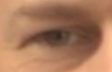
\includegraphics[width=4cm]{image/original.png}
 
\includegraphics[width=4cm]{image/canny_moyenne.png}
 \caption{Image de test et résultat de l'algorithme de Canny avec une moyenne des pixels}
\end{figure}

On voit que cette méthode n'est pas optimale et supprime trop d'informations. De plus,
l'algorithme prend en compte les ombres présentes dans l'image. Nous devons adapter cette méthode
afin de mieux détecter les contours dans les zones que nous souhaitons.

\subsubsection{Avec une moyenne de pixels sur des parties de l'image}

% TODO segmenter une image c'est veut binariser ... mais pas découper 
Plutôt que de prendre la moyenne des pixels sur l'ensemble de l'image de la zone péri-oculaire, nous segmentons l'image
en plusieurs zones dans lesquelles nous calculons la moyenne. Puis nous effectuons l'algorithme
de Canny sur chacune de ces zones. Le résultat nous fournit bien une image dans laquelle l'oeil
est détecté.

\begin{figure}[H]
 \center
 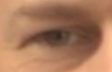
\includegraphics[width=4cm]{image/original.png}
 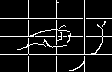
\includegraphics[width=4cm]{image/canny_decomposition.png}
 \caption{Image de test et résultat de l'algorithme de Canny avec division de l'image en 16}
\end{figure}

Avec cette méthode, nous obtenons une image bruitée avec les bords de chaque rectangle utilisé
pour le calcul précédent, car l'algorithme de Canny ne prend pas en compte les bords de l'image
qu'il traite. Avec ce bruit nous ne pouvons pas effectuer une recherche de l'oeil dans
l'image. Il nous faut donc trouver une solution pour supprimer les traits
sans supprimer les contours présents dans l'image résultante.

\subsection{Ouverture des sous-images}

Pour résoudre le problème précédent, nous utilisons deux opérations morphogiques\footnote{filtre non linéaire} :
la dilatation et l'érosion d'une image.\\

La dilatation d'une image est une opération morphologique qui utilise 
un élément structurant afin d'effectuer une convolution de l'image. Si l'un des voisins du pixel traité
est blanc alors celui-ci sera blanc, sinon il sera noir.
Cette opération a pour effet d'élargir une forme et de combler les trous qui peuvent être présents
dans celle-ci. Nous avons également l'opération inverse qui est l'érosion, qui va diminuer la surface de la forme.
Lorsqu'une dilatation est effectuée sur une image en niveau de gris, le pixel traité prend la valeur maximum parmi
ses voisins, et la valeur minimum pour l'érosion.\\

L'ouverture est la combinaison des deux opérations morphologiques vues précédemment, en commençant par 
l'érosion puis la dilatation. Cela a pour effet de fusionner des formes si elles sont proches (dans ce
cas il y a des chances que ce soit le même objet) et de diminuer la largeur de la forme pour 
s'approcher de la forme réelle.\\ 

Afin de supprimer le bruit présent dans l'image de l'oeil après utilisation du filtre de Canny, nous effectuons une ouverture
de chaque sous image.

\begin{figure}[H]
 \center
 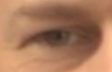
\includegraphics[width=4cm]{image/original.png}
 
\includegraphics[width=4cm]{image/canny_final.png}
 \caption{Image de test et résultat de l'algorithme de Canny avec dilatation puis érosion des sous-images}
\end{figure}

Grâce à ce procédé, nous obtenons une image sans la grille que nous avions précédemment. Cependant,
le bruit dû aux ombres et aux rides ne permet pas encore d'effectuer des traitements pour localiser le centre de l'oeil.
Nous avons un second problème qui est la couleur de peau de l'utilisateur. Nous avons appliqué notre méthode 
sur des personnes ayant des couleurs de peau différentes et les résultats n'étaient pas exploitables (voir annexe p\pageref{resultCanny}).\\ 

Afin de supprimer les bruits dûs aux ombres présentes dans l'image, nous décidons de travailler sur d'autres modèles
colorimétriques comme le HSV\footnote{Hue Saturation Value} dont la composante \enquote{saturation} peut nous
permettre de ne plus prendre en compte les changements importants de luminance.

\subsection{Les modèles Colorimétriques}
Un modèle colorimétrique est une façon de représenter numériquement les couleurs. En général, on sépare ces valeurs en trois groupes, les canaux.
Le modèle colorimétrique le plus connu est le RGB, où on retrouve les canaux rouge, vert et bleu. Les canaux peuvent porter
d'autres informations comme nous allons le voir dans la suite.

\subsubsection{Le modèle HSV}
Le modèle colorimétrique HSV est composé de la teinte\footnote{Hue}, la saturation\footnote{Saturation} et la valeur\footnote{Value}.
La \textit{teinte} correspond à la forme la plus pure des couleurs. La \textit{saturation} est l'intensité de la couleur, plus cette valeur est faible
et plus la couleur semble fade. Et enfin la \textit{valeur} correspond à la luminosité de la couleur, plus cette valeur est petite et plus la
couleur est sombre.

\begin{figure}[H]
 \center
 
\includegraphics[width=4cm]{image/hue.png}
 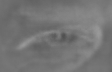
\includegraphics[width=4cm]{image/saturation.png}
 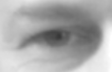
\includegraphics[width=4cm]{image/value.png}
 \caption{Décomposition du modèle HSV}
\end{figure}

Etant donné que notre problème actuel est l'ombre présente dans l'image, nous séparons les trois canaux du modèle HSV. Cela
nous permet de garder la plus appropriée pour nos traitements. Nous ne prendrons pas le troisième canal puisqu'il représente 
la luminosité et que notre problème actuel est dû aux ombres présentes dans l'image. Le canal le plus approprié serait la \textit{saturation}. 
Cependant, lorsque nous appliquons le filtre de Canny sur ce canal, le résultat ne nous permet pas de détecter l'oeil.

\begin{figure}[H]
 \center
 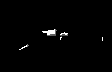
\includegraphics[width=3cm]{image/cannySaturation.png}
 \caption{Résultat du filtre de Canny sur le canal saturation}
\end{figure}

Ce modèle colorimétrique ne nous permet donc pas de détecter l'oeil, car aucun des problèmes que nous avons rencontré
précédemment n'a été résolu. Cependant, après plusieurs recherches, nous avons trouvé une solution qui pourrait résoudre
le problème de la couleur de peau grâce à un autre modèle colorimétrique.

\subsubsection{Le modèle YCbCr}

Nous avons testé un second modèle colorimétrique suite à l'étude des travaux de Evangelos Skodras et Nikolaos Fakotakis\cite{Skodras_2012ieee}.
En effet, leur étude montre que les différentes couleurs de peau de l'homme ont à peu près la même valeur dans deux des
composantes du modèle YCbCr.\\

On peut voir sur le résultat de la décomposition de l'image, que le canal représentant la première chrominance met 
en évidence la pupille de l'oeil.
\begin{figure}[H]
 \center
 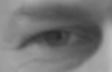
\includegraphics[width=4cm]{image/luminance.png}
 
\includegraphics[width=4cm]{image/chrominance1.png}
 
\includegraphics[width=4cm]{image/chrominance2.png}
 \caption{Décomposition du modèle YCbCr}
\end{figure}

\begin{figure}[H]
 \center
 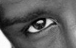
\includegraphics[width=4cm]{image/luminance_black.png}
 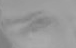
\includegraphics[width=4cm]{image/chrominance1_black.png}
 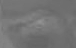
\includegraphics[width=4cm]{image/chrominance2_black.png}
 \caption{Décomposition du modèle YCbCr avec une couleur de peau plus foncée}
\end{figure}

Pour obtenir la valeur des différentes composantes de cet espace colorimétrique à partir
d'une image RGB, il faut effectuer les calculs suivants :
$$Y = 0.299R + 0.587 G + 0.114 B$$
$$Cb = -0.1687R - 0.3313 G + 0.5B + 128$$
$$Cr = 0.5R -0.4187G -0.0813B + 128$$

Nous appliquons ces calculs sur la couleur la plus représentative de la peau des trois modèles
que nous avons pris précédemment, afin de voir si les résultats confirment le fait que la première
chrominance est similaire quelque soit la couleur de peau.

\begin{figure}[H]
 \begin{tabular}{|c|c|c|c|c|c|c|}
  \hline
  couleur de peau & rouge & verte & bleu & luminance(Y) & chrominance 1(Cb) & chrominance 2(Cr)\\
  \hline
  blanc & 234 & 171 & 130 & 185 & 97 & 163 \\
  \hline
  bronzé & 175 & 112 & 95 & 129 & 109 & 161 \\
  \hline
  asiatique & 202 & 143 & 111 & 157 & 102 & 160\\
  \hline
 \end{tabular}
 \caption{Tableau des valeurs des couleurs de peau dans les espaces RGB et YCbCr}
\end{figure}

Nous pouvons voir avec ce tableau que la valeurs des deux chrominances sont très proches quelque soit
la couleur de la peau. Pour la suite des traitements, nous décidons de garder la première chrominance qui semble
varier un peu moins avec le changement de luminosité. En prenant le canal de la première chrominance et en 
prenant un seuil qui semble correct à première vue pour la binarisation, nous obtenons une image comportant la forme de l'oeil au bon endroit.

\begin{figure}[H]
 \center
 
\includegraphics[width=4cm]{image/result_yuv.png}
 \caption{Résultat après traitement sur la chrominance 1}
\end{figure}

Il nous faut maintenant trouver les bons paramètres afin d'obtenir une image binaire qui nous permet d'extraire les 
coordonnées de l'œil.

\subsection{Binarisation de l'image}
Nous souhaitons une image binaire à partir du premier canal de chrominance afin d'y appliquer les blobs. 
Notre but est de retrouver la forme convexe qui correspond à celle de l'œil. Ainsi, le centroïde de cette 
forme nous donne le centre de l'œil.\\

Dans ce but, plusieurs étapes sont nécessaire. D'abord, nous normalisons l'histogramme afin d'utiliser 
tous les niveaux de gris, celà nous permet de travailler sur l'ensemble de l'histogramme quel que soit
image et le visage détecté. Nous préférons faire une normalisation de l'histogramme, plutôt qu'une 
égalisation. En effet, l'égalisation répartit au mieux les niveaux de gris sur l'ensemble de 
la plage de l'hisgramme. Nous souhaitons conserver les modes et les niveaux plus sombres, or l'égalisation 
à pour effet d'étaler les modes de l'histogramme et de rassembler les tons sombres et clairs. À l'inverse, 
la normalisation répartit proportionnellement les niveaux de gris sur toute la plage ().\\


\subsection{Sélection de composantes convexes avec des blobs}
Maintenant que nous obtenons une image binarisée comportant la forme de l'oeil, nous pouvons déterminer où est
positionné son centre. Pour cela nous avons choisi l'utilisation des blobs, afin de résoudre un second 
problème que nous avons rencontré. Lorsque nous effectuons les traitements précédents sur la vidéo, nous avons
parfois des éléments qui perturbent la détection de contour comme des montures de lunettes ou les cheveux de la personne 
filmée. Ces éléments peuvent faire partie des formes que nous récupérons lors de la binarisation.\\ 

Les blobs nous permettent d'étiqueter chaque composante convexe présente dans l'image en annotant
chaque pixel de celle-ci. Si un pixel n'a aucun voisin d'annoté, on lui donne un nouveau numéro et si
l'un de ces voisins est annoté alors il prend le numéro de ce voisin. Nous obtenons ainsi des enveloppes
convexes sur lesquelles nous vérifions qu'elles respectent bien certaines contraintes.\\

Dans notre cas nous avons posé les conditions suivantes :
\begin{itemize}
 \item Le blob de l'oeil est censé être convexe, il ne devrait donc pas y avoir de trous dans le blob
 \item S'il y a plusieurs blobs alors l'oeil devrait être celui qui est le plus proche du centre, étant
 donné que la ROI doit être centré sur l'oeil.
\end{itemize}
Ces conditions nous permettent de supprimer les éléments perturbateurs qui étaient présents dans l'image binaire.
Nous obtenons donc une forme représentant l'oeil, il suffit maintenant de calculer le centre de cette forme
pour obtenir la localisation du centre de l'oeil. Pour cela nous utilisons le calcul du barycentre.